\subsection{Método}

Segundo \citeonline{php5ConceitosProgramacaoEIntegracaoComBancoDeDados}, um
método pode ser definido como sendo as operações que manipulam os dados de uma
classe, ou seja, definem o que as classes podem e sabem fazer, como por exemplo
acelerar um carro modificando o valor de sua propriedade chamada
\textit{velocidade} para um valor crescente em um determinado espaço de tempo.

Os métodos também podem ser chamados de funções membro \cite{c++ComoProgramar}.

Se comparado a programação estruturada um método pode ser considerado como sendo
uma função que está associada a uma classe \cite{programmingPhp}.

\begin{figure}[h!tb]
	\caption{Criação de um Método utilizando a linguagem PHP}
	\label{fig:metodo}

	\centering
	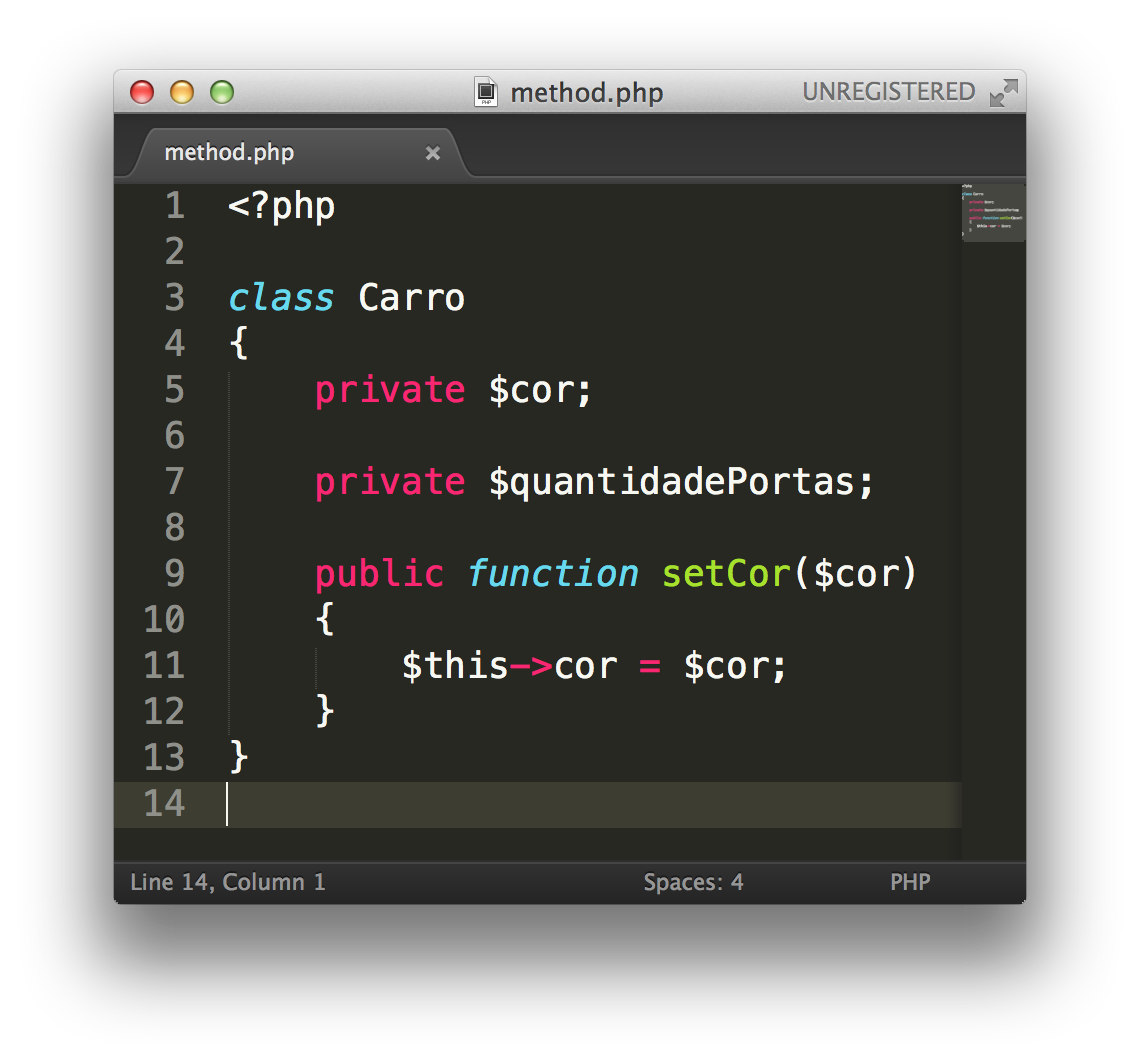
\includegraphics[width=0.75\textwidth]{images/method.png}

	\centering
	\footnotesize Fonte: \fonteOAutor
\end{figure}

\FloatBarrier 	% Este comando impede que as imagens
				% flutuem a partir deste ponto no seu documento

Na sequência, você irá conferir uma explicação referente ao código que foi
apresentado na Figura \ref{fig:metodo}:

\begin{enumerate}[a)]
    \item linha 1: vê-se o início da execução de um bloco de código PHP;
    \item linha 3: define-se uma classe chamada \textit{Carro};
    \item linha 4: informa-se onde inicia o bloco de uma classe;
    \item linha 5 e 7: cria-se duas propriedades para a classe
    \textit{Carro}, são elas: \textit{\$cor} e \textit{\$quantidadePortas};
    \item linha 9: é solicitado para que o interpretador crie um método
    cuja visibilidade seja pública e definisse que este método será identificado
    pelo nome \textit{setCor}.
    Além disso, informasse que este método deve receber um parâmetro (um valor
    que  irá configurar a propriedade de uma classe);
    \item linha 10: define-se onde inicia o bloco cujo escopo
    corresponda ao método \textit{setCor};
    \item linha 11: utilizou-se uma variável especial chamada
    \textit{\$this}, esta variável permite acessar qualquer propriedade ou
    método dentro da própria classe ou \textit{superclasse}; depois, usou-se
    o operador de acesso a um objeto (representado pelo símbolo \textbf{->}); em
    seguida, informa-se ao interpretado do \acs{PHP}, a necessidade de manipular
    o valor da propriedade \textit{cor}, sendo que, ela deverá receber o valor
    informado como parâmetro para o método \textit{setCor};
    \item linha 12: define-se onde termina o bloco que corresponde ao
    método \textit{setCor};
    \item linha 13: informa-se o encerramento do bloco de uma classe.
\end{enumerate}

Isto permite que de fora da classe carro outro objeto configure a cor de um
veículo passando uma mensagem ao objeto carro com a cor solicitada. Na Figura
\ref{fig:chamadaMetodo} será exibido um exemplo desta situação:


\begin{figure}[h!tb]
	\caption{Chamada de um Método utilizando a linguagem PHP}
	\label{fig:chamadaMetodo}

	\centering
	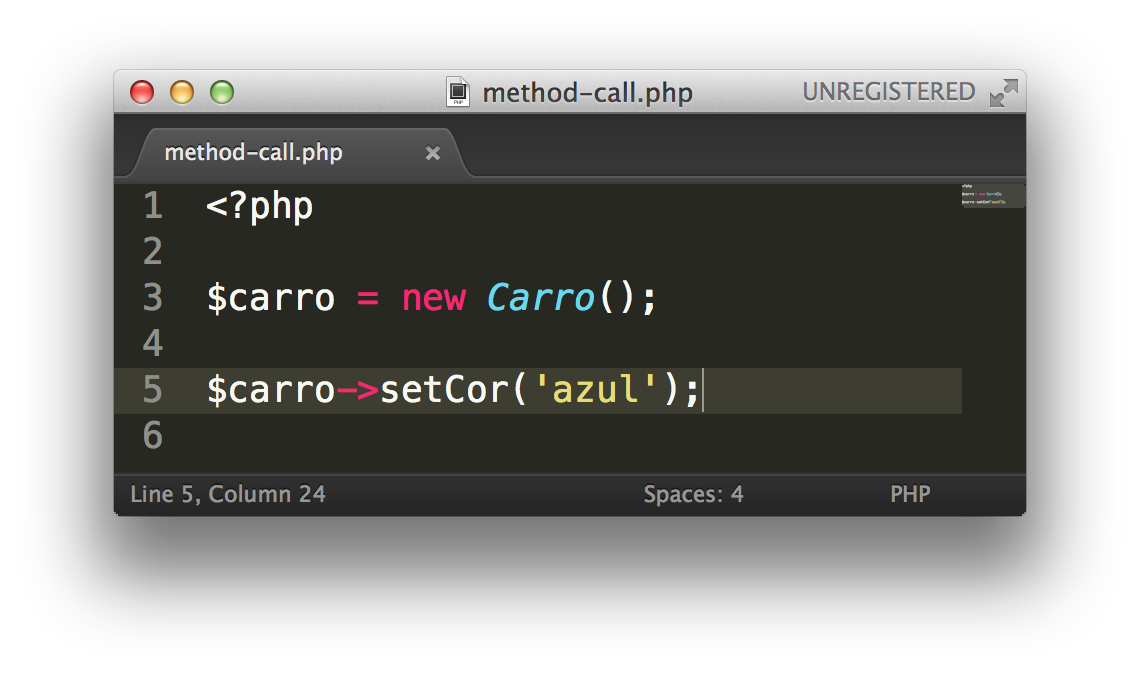
\includegraphics[width=0.75\textwidth]{images/method-call.png}

	\centering
	\footnotesize Fonte: \fonteOAutor
\end{figure}

\FloatBarrier 	% Este comando impede que as imagens
				% flutuem a partir deste ponto no seu documento

Abaixo, você irá conferir uma explicação referente ao código que foi
apresentado na Figura \ref{fig:chamadaMetodo}:

\begin{enumerate}[a)]
    \item linha 1: tem-se o início da execução de um bloco de código
    PHP;
    \item linha 2: ocorre a criação de um objeto do tipo \textit{Carro};
    \item linha 5: realiza-se a chamada de um método chamado
    \textit{setCor}, sendo que, informa-se um parâmetro para ele, que na
    linguagem PHP representa uma \textit{string} (cadeira de caracteres). Logo,
    configura-se o valor da propriedade \textit{cor} da classe \textit{Carro}
    para receber o valor \textit{azul}.
\end{enumerate}